\documentclass[12pt,fleqn]{article}
\setlength{\parindent}{0pt}
\usepackage{graphicx}
\usepackage{cancel}
\usepackage{listings}
\usepackage[latin5]{inputenc}
\usepackage{color}
\setlength{\parskip}{8pt}
\setlength{\parsep}{0pt}
\setlength{\headsep}{0pt}
\setlength{\topskip}{0pt}
\setlength{\topmargin}{0pt}
\setlength{\topsep}{0pt}
\setlength{\partopsep}{0pt}
\setlength{\mathindent}{0cm}

\begin{document}
Ders 1

Bir Kismi Turevsel Denklem (PDE) cok degiskenli bilinmeyen bir fonksiyon ve
o fonksiyonun kismi turevleri arasinda kurulan bir iliskidir. 

Ornek 

\[ u = u(x,t) \]

olmak uzere

\[ \frac{\partial u}{\partial x} + \frac{\partial u}{\partial t} = 0\]

denklemi bir PDE'dir. Cozum bir tek sayisal sonuc degil, bir
fonksiyondur. Dusunelim, mesela $f$ fonksiyonu tek degiskenli ve turevi
alinabilir bir fonksiyon ise

\[ u(x,t) = f(x-t) \]

cozumdur diyebilir miyiz? Yani cozum $f(x-t)$ olabilir mi? Kontrol edelim 

\[ u_x = f'(x-t) \]

\[ u_t = -f'(x-t) \]

Bu iki kismi turev toplaninca sifir cikar, yani sonuc ustte tanimli PDE'ye
uyar. Bu genel tanima uyan bir suru fonksiyon vardir, mesela 

\[ u(x,t) = (x-t)^2 \]

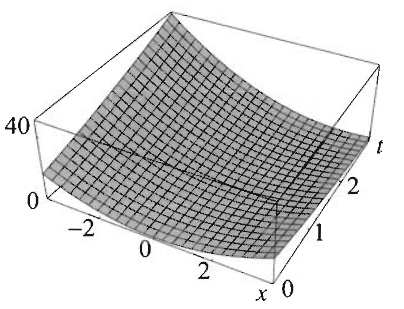
\includegraphics[height=4cm]{1_01.png}

\[ u(x,t) = e^{-(x-t)^2} \]

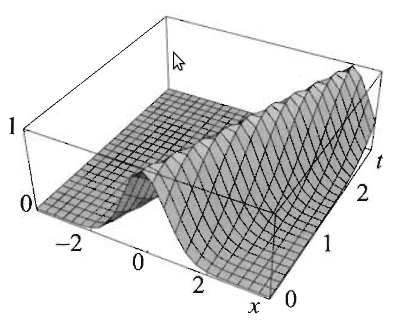
\includegraphics[height=4cm]{1_02.png}

\[ u(x,t) = 3sin(x-t) \]

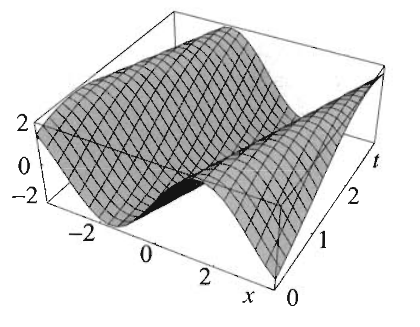
\includegraphics[height=4cm]{1_4.png}

Not: Burada $f$'i bir $f(z)$ olarak gorebiliriz, bu fonksiyona $(x-y)$
geciliyor, yani bir icice fonksiyon ortaya cikiyor. O zaman ustteki formlar
aslinda $f(z) = z^2$, ve $e^{-z^2}$ seklinde. Tabii kismi turevler ile
turev alinca Zincirleme Kanunu devreye girmelidir ve gecilen degerlerin,
``fonksiyonlarin'' da turevi alinmalidir, vs. 

Yani ustteki sonuc aslinda diyor ki $x-t$ seklinde hep beraber olmak uzere
bu ikiliyi kullanan herhangi bir fonksiyon, ustteki PDE'nin
cozumudur. Bu sekilde cozum birden fazla fonksiyon oluyor, ve bunlarin
birbirinden ne kadar farkli olabildigi gostermeye calistigimiz noktalardan
biri. 

Ustteki PDE bir tasinim (advection) ornegidir, ve 1. seviye lineer homojen
bir denklemdir. 1. seviye en yuksek turev seviyesinin seviyesine isaret
eder, lineer homojen ise tum cozumlerin lineer bir sekildeki kombinasyonu
yine bir cozumdur anlamina gelir. Ustteki PDE icin ne kadar cesitli
cozumler olabildigini gorduk, onlarin kombinasyonlariyla bu cesitlerin daha
da artacagini dusunebiliriz. kiyasla soyle bir ODE icin

\[  y' - y  = 0\]

icin cozumler

\[ y = Ae^x \]

denklemidir Tek bir cozume indirgemek icin baslangic sarti mesela $y(0) =
2$ 
veririz ve oradan tek cozum $y = 2e^x$ buluruz. 

Ornek PDE'miz icin de, benzer sekilde, tek bir fonksiyonu bulmak icin
baslangic, ya da sinir sartlari koymaliyiz. 

Ornek

Ornek PDE cozumleri arasinda hangisi x ekseni boyunca $u = e^{-x^2}$
sartini tatmin eder? 

$u = e^{-x^2}$ demek, $u(x,0)$ demektir, cunku $t$ yoktur. Cozumlerimizi
teker teker gozden gecirirsek, $u(x,0)$ denklemi $u = e^{-x^2}$ olan
cozum

\[ u(x,t) =  e^{-(x-t)^2} \]

cozumudur. Gorsel olarak durumu canlandirmak gerekirse, $t$'yi bir zaman
degiskeni olarak kabul edelim, ve 

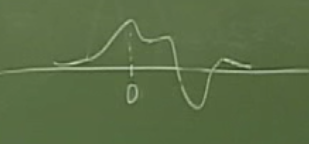
\includegraphics[height=2cm]{1_3.png}

her $t$ degerinde o anda $u$'nun $x$ uzerinde dusen yansimasinin bir
fotografini cekiyoruz sanki, ustteki resimde soldaki $t=0$ anindaki
mesela. 

Devam edelim. Ornek 1 icin bir suru cozumden bahsettik ama bu cozumleri
nasil turettigimizi soylemedik. Ayrica bu ornekte ``tum mumkun cozumleri''
bulup bulmadigimizi da soylemedik. Simdi gosterecegimiz islemler hakikaten
tum cozumleri buldugumuzu gosterecek, ve akillica kullanilabilecek bir
degisken degistirme (change of variables) tekniginin bir problemi
basitlestirmekte nasil faydali olacagini anlatmaya ugrasacak. 

Ornek

Ustteki PDE'yi lineer degisken degisimi kullanarak bir ODE'ye indirgemeye
ugrasacagiz. Diyelim ki

\[ \alpha = a x + b t \]

\[ \beta = cx + dt \]

Kismi turevler $u_x$ ve $u_t$ su sekilde genisletilebilir

\[ u_x = 
\frac{\partial u}{\partial \alpha}\frac{\partial \alpha}{\partial x}  +
\frac{\partial u}{\partial \beta}\frac{\partial \beta}{\partial x} 
\]


\[ u_t = 
\frac{\partial u}{\partial \alpha}\frac{\partial \alpha}{\partial t}  +
\frac{\partial u}{\partial \beta}\frac{\partial \beta}{\partial t} 
\]

Ilk bastaki degisken degisimine gore bazi kismi turevler soyle:

\[ \frac{\partial \alpha}{\partial x} = a , \ \frac{\partial \alpha}{\partial t} = b, \ \frac{\partial \beta}{\partial x} = c , \
\frac{\partial \beta}{\partial t} = d 
\]

Bunlari $u_x$ ve $u_t$ icinde yerlerine gecirirsek,

\[ u_x = 
\frac{\partial u}{\partial \alpha} a +
\frac{\partial u}{\partial \beta} c
\]

\[ u_t = 
\frac{\partial u}{\partial \alpha} b +
\frac{\partial u}{\partial \beta} d
\]

Ustteki iki kismi turevi ana PDE'de yerine koyarsak

\[ \frac{\partial u}{\partial x} + \frac{\partial u}{\partial t} = 0\]

soyle olur

\[ 
\frac{\partial u}{\partial \alpha} a  +
\frac{\partial u}{\partial \beta} c + 
\frac{\partial u}{\partial \alpha} b + 
\frac{\partial u}{\partial \beta} d = 0
\]

Benzer terimleri gruplayalim

\[ 
\frac{\partial u}{\partial \alpha} (a+b)
\frac{\partial u}{\partial \beta} (c+d) = 0
\]

Simdi oyle $a,b,c,d$ degerleri secelim ki bir kismi turev yokolsun. Mesela 

\[ a = 1, b = 0, c=1, d=-1 \]


O zaman 

\[ \frac{\partial u}{\partial \alpha} = 0 \]

kalir. Bu artik bir basit diferansiyel denklemdir, cozum icin entegral
aliriz, 

\[ u = C(\beta) \]

Unutmayalim, sifirin entegrali bir sabittir, ama $u$ birden fazla degiskene
sahip oldugu icin bu ``sabitin'' $\beta$ icermesi gerekir. $C(\beta)$,
$\alpha$'ya gore bir sabittir. 

$C(\beta)$'yi daha somutlastiralim, 

\[ \beta = cx + dt \]
 
demistik, ayrica $c=1,d=-1$. O zaman cozum

\[ u = C(x-t) \]

Bu da basta buldugumuz cozum ile ayni zaten. 






\end{document}
